% \begin{savequote}[75mm]
% Nulla facilisi. In vel sem. Morbi id urna in diam dignissim feugiat. Proin molestie tortor eu velit. Aliquam erat volutpat. Nullam ultrices, diam tempus vulputate egestas, eros pede varius leo.
% \qauthor{Quoteauthor Lastname}
% \end{savequote}

\chapter{AAV fitness landscape reveals capsid design principles and a new viral gene}

% \newthought{There's something to be said} for having a good opening line. Morbi commodo, ipsum sed pharetra gravida, orci  $x = 1/\alpha$ magna rhoncus neque, id pulvinar odio lorem non turpis. Nullam sit amet enim. Suspendisse id velit vitae ligula volutpat condimentum. Aliquam erat volutpat. Sed quis velit. Nulla facilisi. Nulla libero. Vivamus pharetra posuere sapien. Nam consectetuer. Sed aliquam, nunc eget euismod ullamcorper, lectus nunc ullamcorper orci, fermentum bibendum enim nibh eget ipsum. Donec porttitor ligula eu dolor. Maecenas vitae nulla consequat libero cursus venenatis. Nam magna enim, accumsan eu, blandit sed, blandit a, eros.
% $$\zeta = \frac{1039}{\pi}$$


% For an example of a full page figure, see Fig.~\ref{fig:myFullPageFigure}.

\newthought{Since the discovery of AAV} in 1965 \cite{ATCHISON1965}, efforts to map and manipulate its complex genome have enabled the widespread use of AAV vectors for therapeutic in vivo gene delivery \cite{Grimm2015, Hastie2015, Srivastava1983, Pereira1997, Wu2006,Russell2017}. AAV capsids have been utilized for in vivo delivery to a wide variety of tissues, but the transduction efficiency of natural capsids is often limiting for therapeutic purposes \cite{Wu2006}. Furthermore, the engineering of enhanced capsids has proven challenging due to the complexity of its genotype-phenotype relationships and the many properties of the capsid that must be simultaneously optimized (9). 

To better understand AAV and to inform capsid engineering efforts, we generated all possible single codon mutants at every position within the AAV2 Cap gene. AAV2 is the most studied AAV serotype, and is also the first gene therapy FDA approved for use in humans[REF luxturna Ph3 trial]. Additionally, the AAV2 Rep gene and ITR sequence are used for recombinant production in most gene therapy applications. In contrast to previous works studying AAV capsids (as well other proteins) which focused on amino acid level changes, we include all synonymous codons for each amino acid to enable detection of non-coding elements and frame-shifted ORFs. We included wild-type (WT) AAV2 sequences and null mutants (stop codon substitutions) in the library as positive and negative controls, respectively. In addition to all possible codon substitutions, we also included all single codon insertions and deletions. After assembly, the final plasmid contained the full length capsid gene with an upstream promoter and a downstream barcode, all flanked by inverted terminal repeats (ITRs) (Fig. 1a, Fig. S1a,b). Importantly, barcoding of the library enabled us to efficiently measure the frequency of mutants at all positions within the gene from a single experiment via high-throughput sequencing (Fig S1b). The total library design contained 29,400 amino acid mutants derived from 91,875 codon mutants, with each codon mutant represented by at least 2 unique barcodes, for a total of 183,750 variants (see Methods for a full description). Using NGS, we confirmed that >99.1\% of all expected codon mutants were generated in our initial plasmid library. To obtain adequate sequencing coverage of the entire library, we developed a novel barcode ligation method that incorporates multiple barcodes into a single Illumina read, thereby increasing read depth by approximately 7-fold (Fig. S1c).

\begin{figure}
\includegraphics[width=\textwidth]{figures/20190610_AAV2_fig1_PO_working_v2.pdf}
\caption[Multiplexed in vitro characterization of capsid transduction in a neutralizing antibody assay recapitulates A20 binding residue importance]{Multiplexed in vitro characterization of capsid transduction in a neutralizing antibody assay recapitulates A20 binding residue importance 
a, Neutralization assay: Virus library is incubated with A20 antibody and then added to cells with adenovirus. 6 days later virus is collected and barcodes are sequenced. b, distribution of selection values after neutralization. c, fraction of residues above the positive selection cutoff which are known A20 interactors. d, Selection values for substitutions and deletions of all positions contacting in A20-AAV2 cryo-em structure.]
\label{fig:Figure 1}}
\end{figure}

To understand how Cap sequence changes impact virus production (e.g. assembly and packaging) we transfected the pooled plasmid library into HEK-293T cells to produce recombinant AAV and then purified the resulting virus (Fig. 1a). We first assessed the impact of any given amino acid change by calculating the normalized enrichment of mutants (“selection”) compared to WT within the resulting pool (Fig. 1b, Methods), summing counts across all synonymous codons. We generated libraries in two contexts: as recombinant AAV (pCMV, with Cap driven by CMV promoter) or in the WT-AAV context (pRep, with full length Rep upstream). In both cases, fitness measurements across independent transfection replicates were highly correlated (R=0.91 for pCMV, R=0.99 for pRep, p<10-20) (Fig. S2a S2b) and positive controls (WT replicates) were tightly distributed (Fig. 1c, Fig. S3). Selection values were generally stronger in the rRep context, possibly because of the ability of these AAVs to self-replicate (Methods). In pCMV context, only VP3 is essential for capsid assembly (15,16), thus we expected nonsense mutations in the VP3 region to be most strongly depleted from the packaged library. Indeed, these mutations were depleted 30-fold relative to WT capsids (p<10-20) (Fig. 1c). Nonsense mutations within VP1 and VP2 had a lesser effect on packaging, showing only 10 fold depletion relative to WT (p<10-20) (Fig. 1c). 

We examined positions in the capsid for their capacity to tolerate mutations. Location within the capsid structure (17) was correlated with sensitivity to insertions and deletions: mutations at positions buried within the protein were more deleterious, as were those near the 5-fold axis of symmetry, while those exposed to the outer surface and near the 3-fold axis of symmetry were better tolerated (Fig. 1d and 1e). Similarly, variable regions identified from evolutionary capsid alignments (18,19) were more mutable than non-variable regions (p<10-20) (Fig. 1e). Outside of the variable regions, positions tended to better tolerate substitution to amino acids found within other serotypes than substitutions to amino acids never observed across a set of commonly studied AAVs (p<10-20) (Fig. 1f). In contrast to alanine scanning, comprehensive mutagenesis allowed us to observe the effects of different amino acid properties on function: positively charged residues tended to be deleterious across all positions while negatively charged residues were most beneficial within outward facing capsid residues, especially near the 3-fold axis of symmetry. Mutations to methionine (ATG) were deleterious throughout the VP1 coding region (Fig. 1d), likely due to the initiation of translation at this position resulting in reduced production of VP2 and VP3 monomers or because these truncated VP1 products inhibit capsid formation. 

\begin{figure}
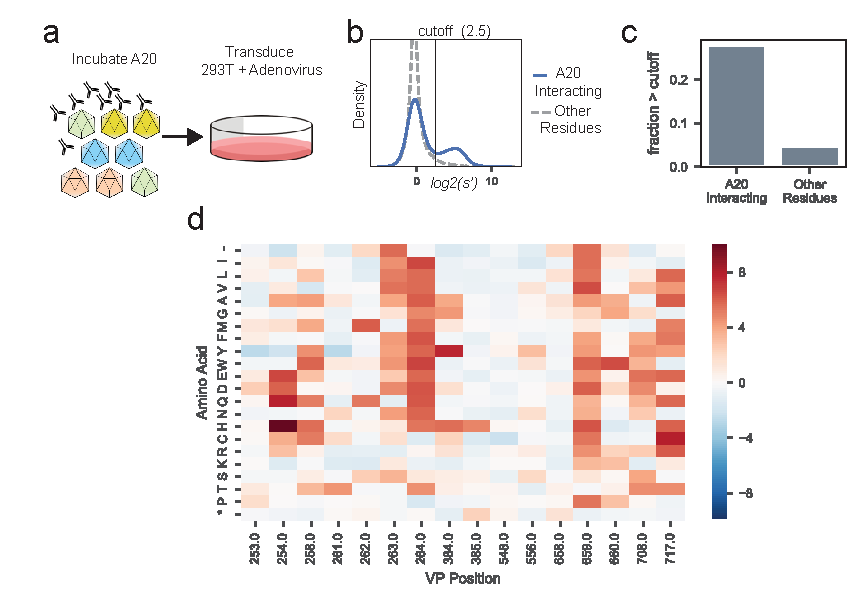
\includegraphics[width=\textwidth]{figures/20190405_x01_A20_only_revisions.pdf}
\caption[Multiplexed in vitro characterization of capsid transduction in a neutralizing antibody assay recapitulates A20 binding residue importance]{Multiplexed in vitro characterization of capsid transduction in a neutralizing antibody assay recapitulates A20 binding residue importance 
a, Neutralization assay: Virus library is incubated with A20 antibody and then added to cells with adenovirus. 6 days later virus is collected and barcodes are sequenced. b, distribution of selection values after neutralization. c, fraction of residues above the positive selection cutoff which are known A20 interactors. d, Selection values for substitutions and deletions of all positions contacting in A20-AAV2 cryo-em structure]
\label{fig:Figure 2}}
\end{figure}

Utilizing the self-replicative ability of pRep library, we measured mutations that enable escape of neutralization by the A20 monoclonal antibody, whose binding epitope on the capsid surface has been identified through cryo-EM20 (Fig. S4a). Single amino acid changes enabled escape from neutralization, with the location of escape mutations matching well with the position of the known epitope (p<10-20) (Fig. S4b and S4c). Some mutants were much more potent at escape than other mutants at the same location (Fig. S4d), demonstrating the ability of this approach to identify mutations with enhanced potential for overcoming pre-existing immunity.  

With the pCMV library, we measured capsid thermostability by incubating the library at a range of temperatures and digesting the genomes of thermolabile capsids (Fig. S5a). The storage and stability of AAV formations for gene therapy is an important therapeutic concern, and while natural and engineered capsid serotypes differ widely in their thermostability 21–23, the basis for this variability is unclear. Strikingly, mutations at the 3-fold axis decreased thermostability (p<10-8) suggesting that capsid disassembly could initiate at these positions (Fig. S5b-d).

\begin{figure}
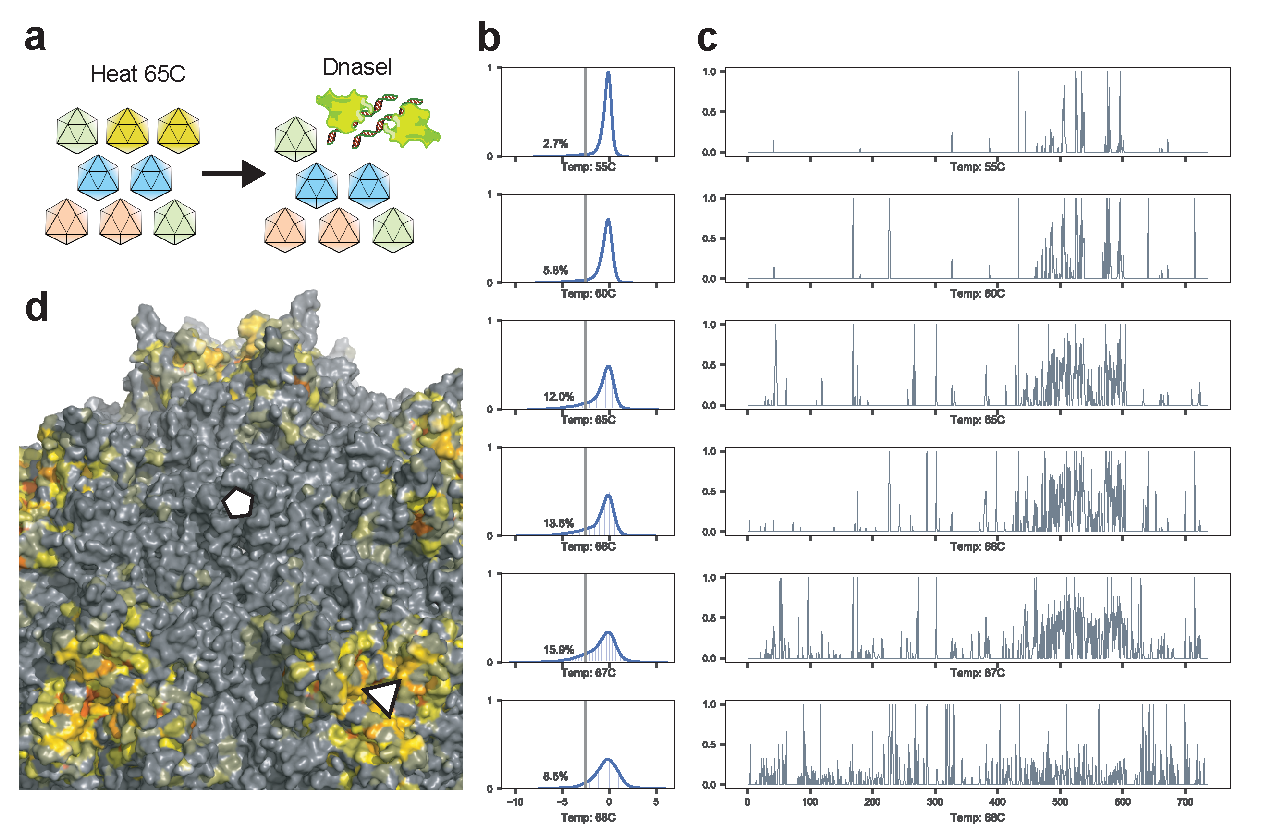
\includegraphics[width=1\linewidth]{figures/20181130_supp4_tmonly.pdf}
\caption[Multiplexed in vitro characterization of capsid thermostability and transduction in a neutralizing antibody assay reveals dominant structural-function relationships.]{Multiplexed in vitro characterization of capsid thermostability and transduction in a neutralizing antibody assay reveals dominant structural-function relationships.
a, Thermal stability assay. b, Left: distribution of selection values after heating to a range of temperatures; c, fraction of destabilized mutants (below selection cutoff) at each position. d, Fraction of destabilized mutants in thermostability assay plotted on capsid structure; yellow-red color indicates positions with higher fractions of mutants being destabilized; triangle: 3-fold axis, pentagon: 5-fold axis.
\label{fig:Figure 3}}
\end{figure}

Moving on to better understand how capsid mutations affect AAV delivery properties in vivo, we administered 1012 vector genomes (vg) of the pCMV virus library to each of eight mice through retro-orbital injection. Blood was collected one hour after injection and animals were sacrificed 18 days later. Tissue samples from the spleen, liver, kidney, heart, and lung were collected, virus genomes were purified from each tissue, and their barcodes sequenced (Fig. 2a). Selection values from mouse and virus replicates within tissue samples were well correlated (Fig SXa, while correlation values across tissues were often divergent (Fig SXb), indicating different mutants contained distinct biodistribution profiles. To both validate and assess the replicability of our findings, we chose 5 mutants from our library which displayed divergent biodistribution profiles and compared our library-based measurements with those obtained by producing and assaying each capsid individually (N=3 mice/mutant, Methods). The individual capsid biodistribution ratios (mutant/WT) as measured by qPCR significantly correlated with library-based measurements (R=.75, p<10-14) (Fig. 2b), confirming the fidelity of our multiplexed in vivo library assay. 

\begin{figure}
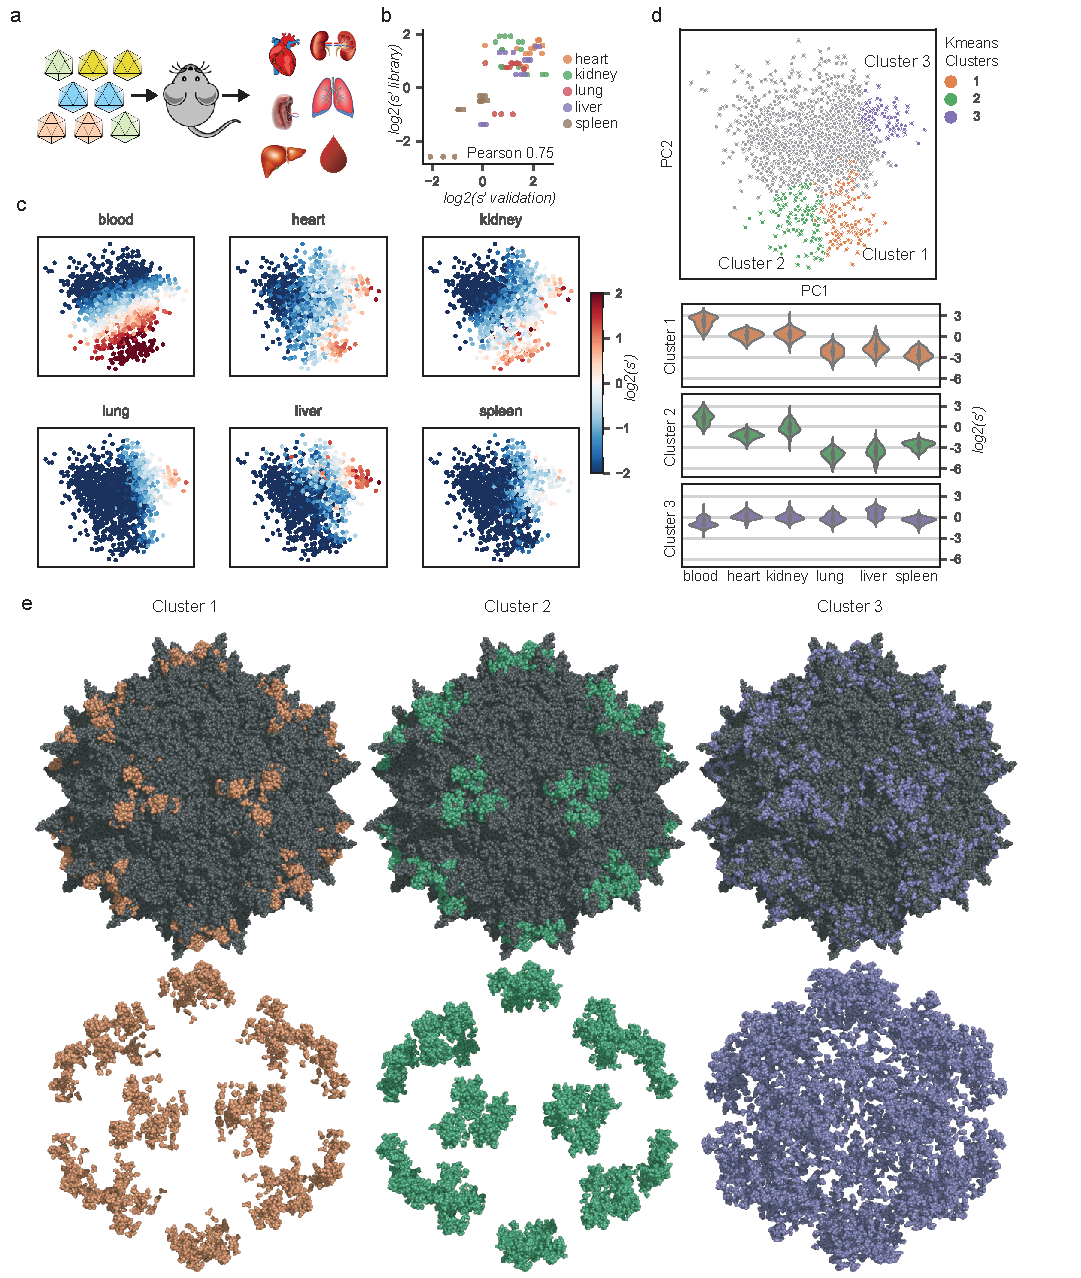
\includegraphics[width=1\linewidth]{figures/20190604_AAV2_fig3_mouse_PO_working_v4.pdf}
\caption[Analyzing mutant biodistribution to major organs in mice reveals major trends affecting in vivo delivery.]{Analyzing mutant biodistribution to major organs in mice reveals major trends affecting in vivo delivery. (A) Biodistribution assay. (B) Mutant in vivo selection values in library format (y-axis) vs selection value in individual validation assays (x-axis) (C) Projection of individual mutants onto PC1 (x-axis) and PC2 (y-axis) derived from PCA, color is selection value for a given tissue. (D) Classification of mutants on PC1-PC2 plane. Lower plots show average selection values of mutants in each Class. (E) Position of mutants contained in each Class colored on capsid crystal structure, top: full capsid, bottom: only showing residues from each class.
\label{fig:Figure 4}}
\end{figure}

Principal component analysis (PCA) applied to the mutant tissue distribution data revealed patterns of mutants with distinct sequence-tropism relationships. Notably, the first two principal components (PCs) explained  \{80\%\} of the variance in mutation tropism profiles. Mutants spanned a continuum of component values; using k-means we identified three mutant clusters with distinct biodistribution profiles (Fig. 2c and 2d, Fig SX). Intriguingly, the 3D-structural locations of each cluster were also different: mutants from Cluster 1 and 2 occurred in tight patches on the capsid surface, mainly near the 3-fold axis, while Cluster 3 mutations were dispersed in buried positions throughout the capsid (Fig. 2e). Cluster 1 mutants included the R585 and R588 mutants(20,21) which were depleted from the liver and enriched in the blood, as expected. Cluster 2 mutants were depleted in heart but enriched in the blood and kidney, indicating a potential difference in viral processing from Cluster 1. Class 3 mutants were depleted from the blood and spleen, and enriched across all other tissues. While many capsid engineering efforts have focused on externally exposed positions[Cite Perabo 2003, Muller 2003, Marsic 2014], these results show that buried positions also play an important role in tuning tropism. Importantly, by narrowing down the number of candidate mutations to those that are viable for production and that affect biodistribution, these data inform the design of combinatorial libraries for enhanced tissue targeting without the loss in viability that typically occurs for randomly mutated libraries [cite the perspective I wrote with George, which now makes this argument for us]. 

\begin{figure}
\includegraphics[width=1\linewidth]{figures/20190402_AAV2_fig4_genez_PO_library_v2.pdf}
\caption[Discovery of a membrane-associated accessory protein (MAAP) expressed from the VP1 region]{Discovery of a membrane-associated accessory protein (MAAP) expressed from the VP1 region. (A) Assay for viral production. (B) Top: effect on production for mutations creating stops and non-stops in the +1 frame; red: +1 frame stop codons, gray: codons synonymous in Cap to the red points but without creating stops in the +1 frame, lines are moving average across 10 nearest positions. Bottom: p-value, calculating the probability of the observed difference in selection coefficients of +1 frame stops and non-stops for a moving window of 10 positions, compared to a random synonymously shuffled null model. (C) Western blot of MAAP-3xFlag and negative controls, stained with M2 anti-Flag HRP antibody. Top band is anti-GAPDH loading control. (D) Indicating membrane-association: confocal imaging of HEK293T cells transfected with Rep+MAAP-GFP, pHelper, AAV2-Cap and mKate; blue: membrane stain, green: GFP. 
\label{fig:Figure 5}}
\end{figure}

One advantage of our comprehensive and unbiased codon scanning approach to library generation is the potential to detect previously unknown gene products and other genetic elements. In particular, functions independent of coding for Cap should manifest as fitness differences among synonymous codons. We devised a Frameshift Score (FS) to detect the presence of frameshifted ORFs by comparing the differences in fitness observed among synonymous mutants to the presence or absence of stop codons in alternative reading frames (Methods). Using selection coefficients from the AAV production assay, we evaluated this metric across the Assembly Activating Protein (AAP), a known frameshifted ORF, and observed a significant FS in the +1 frame (Fig. 3a and 3b), as expected given AAP’s essential role in AAV2 capsid assembly (3,16). Other frameshifted ORFs beyond AAP, such as the X-gene, have been proposed (22). However, we detected no highly significant FS for positions within the X-gene (mean p>.28).

To search for additional frameshifted ORFs, we used this approach to explore the entirety of the Cap gene sequence and detected a highly significant FS representing a novel frameshifted ORF within the +1 frame of the VP1 region (Fig. 3b). Guided by differences in fitness for synonymous codons of Cap, we identified Cap nt 80-439 (VP positions 27-147) as the most likely location of the new ORF. We hypothesized that the ORF starts with CTG, a non-canonical start codon (similar to AAP). Supporting this hypothesis, all mutations to Cap P27(CCT) were deleterious, except for those ending in CT, which preserve the frameshifted ORF’s CTG start codon (Fig. S6a). In this frame, translation continues until reaching a TAG stop codon at Cap nt 437-439, creating a protein 119 amino acids in length. 

This novel ORF’s start and stop codons are conserved across most other serotypes, suggesting a real and conserved function. By aligning the nucleotide sequences of AAV capsid serotypes 1-9, Rh8, Rh10 and Rh32, we observed that the CTG start codon is conserved in all but AAV5 (Fig. S8). At the C-terminus, all serotypes contain a stop codon at the same aligned position, except AAV5, which has a stop codon one position earlier (Fig. S9). Dual sequence constraints from the capsid protein and this ORF help to explain the strikingly high degree of conservation observed for this region, even outside of the VP1 PLA2 domain (Fig. S8 \& 9). Notably, NCBI pBLAST and psiBLAST of the ORF amino acid sequence against the non-redundant protein database returned no proteins with significant homology.

\begin{figure}
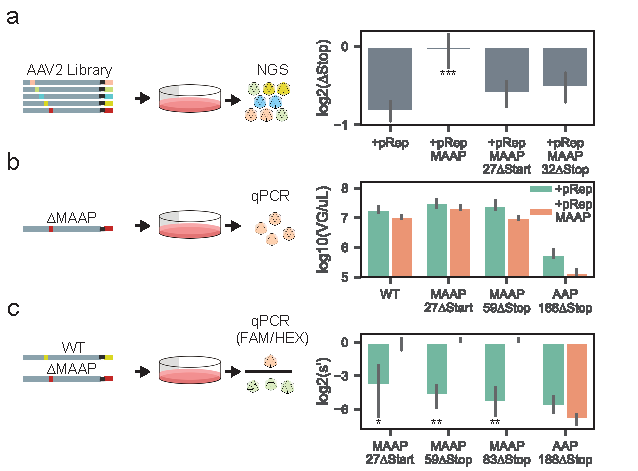
\includegraphics[width=1\linewidth]{figures/20190604_fig7_library_complement.pdf}
\caption[MAAP functions through competitive exclusion]{MAAP functions through competitive exclusion. (A) Assay for viral production. (B) Top: effect on production for mutations creating stops and non-stops in the +1 frame; red: +1 frame stop codons, gray: codons synonymous in Cap to the red points but without creating stops in the +1 frame, lines are moving average across 10 nearest positions. Bottom: p-value, calculating the probability of the observed difference in selection coefficients of +1 frame stops and non-stops for a moving window of 10 positions, compared to a random synonymously shuffled null model. (C) Western blot of MAAP-3xFlag and negative controls, stained with M2 anti-Flag HRP antibody. Top band is anti-GAPDH loading control. (D) Indicating membrane-association: confocal imaging of HEK293T cells transfected with Rep+MAAP-GFP, pHelper, AAV2-Cap and mKate; blue: membrane stain, green: GFP. 
\label{fig:Figure 4}}
\end{figure}

Toward confirming the translation of the ORF in its native context, we modified a Rep-Cap expression plasmid by adding a 3x-FLAG tag to the predicted C-terminus, deleting downstream regions of Cap, and mutating the VP1 start codon. This plasmid was co-transfected into HEK-293T cells together with the pHelper plasmid containing Adenovirus-derived genes that activate transcription from AAV promoters within the Rep gene (12). Through western blotting, we confirmed the presence of a protein migrating near the expected size of 16 kDa (Fig. 3c, Fig. S6b). For negative controls, a synonymous change to Cap that mutated the hypothesized CTG start codon (∆Start: P27P[CCT → CCC]) ablated the primary protein product, as did a Cap mutation creating an early stop codon (∆Stop: P32V[GGT → ATA]) (Fig. 3c, Fig. S6b). The western blot displayed a smaller product for the ∆MAAP mutants, indicating the ability of downstream positions to also initiate translation (Fig. 3c Fig. S6b). AAV2 capsids assemble in the nucleolus (23), but intriguingly, anti-FLAG immunofluorescence imaging revealed that the novel protein was excluded from the nucleus and membrane-associated (Fig X). No AAV proteins are known to associate with the outer membrane, so we independently validated this finding by replacing the FLAG tag with a C-terminal GFP fusion, additionally testing with the MAAP sequences derived from AAV5, AAV8 and AAV9, and producing MAAP both with and without Cap. In all cases the protein was associated with cell membrane (Fig. 3d, Fig. S6c and S7). Based on these observations, we propose the name “membrane-associated accessory protein” (MAAP).

To better understand the functional role of MAAP in our viral production assay, we repeated the production experiment but this time supplemented the library a plasmid containing both Rep and MAAP (Rep+MAAP), in order to express MAAP in trans. Negative controls were also included: Rep only, Rep+MAAP∆Start, and Rep+MAAP∆Stop. The addition of MAAP in trans rescued the packaging abilities of VP mutants containing stop codons within MAAP (p<1e-5) (Fig. 4a). Importantly, MAAP stop codon mutants were not rescued by the negative controls. These results show that MAAP functions separate from any effect in cis within the Cap gene.

We attempted to reconcile the deleterious effects of MAAP mutants on production with previous reports that the entire VP1 region is not essential for capsid assembly[REF Kleinschmidt AAP PNAS paper]. We tested whether mutating MAAP reduced the titer of AAV production when using individual null mutants, both with and without functional MAAP provided in trans. In line with previous reports, MAAP mutants did not significantly reduce production titer (Fig 4b), indicating that MAAP is not essential for capsid assembly. However, when we assayed MAAP mutants in head to head competition with WT (simultaneously transfecting both variants in a single dish), MAAP mutants were strongly deleterious relative to WT unless complemented in trans with functional MAAP (Fig 4c). Indeed, our original large library production experiment where we discovered MAAP likewise pit mutants against each other. These findings demonstrate that MAAP function manifests in a competitive environment. 

Further studies will be required to determine the mechanism of competitive exclusion for MAAP. This capability may help to explain the surprisingly high genome-capsid coupling observed for libraries of engineered AAV capsids[ref Nonnenmacher/Weber paper]. Furthermore, since MAAP is likely present in all AAV capsids in use today for gene therapy, production of these therapies could potentially benefit from an improved understanding MAAP’s function, in HEK293T cells and beyond. 

Together these results demonstrate the power of fitness landscapes for deciphering complex genetic functions and for identifying major trends relevant for bioengineering. Outside of AAV, these approaches can be used to discover cryptic genes in other viruses and organisms. Within AAV, a similar approach can be applied to engineering of Rep for modulating genome replication and packaging, and to optimization of AAV transgene payloads for high-titer production and cell-specific expression. These data and the design principles we have identified will guide the engineering of AAV capsids for enhanced in vivo delivery, on the road to developing new gene therapies.



\section{Methods}

\subsection{Library Construction}
Oligos were synthesized as 230mers on an Agilent oligo array (Fig. S1) The capsid gene was divided into 18 tiles spanning the entire gene. Individual primers designed for minimal cross reactivity were added to both ends of the oligo and used for individual amplification of each of the tile pools individually. Library cloning was performed in a three successive steps (Fig. S1). First, the tile was cloned into a linearized backbone (approx 1ug per reaction) using Golden Gate Assembly (GGA), utilizing BbsI-HF and T4 DNA ligase (2*106 U/ml, NEB) in a 100 uL reaction. The reaction was cycled 100x (16C for 5 min then 37C for 5 min), then heat inactivated. This material was then ethanol precipitated and dissolved in 2uL TE. To this, 50uL of electrocompetent cells were added (Lucigen ELITE 10G) and electroporated (Bio-rad MicroPulser) on EC1 settings. The cells were recovered in Lucigen recovery media for 1 hour at 37C, after which media with selective antibiotic (25mL) was added and the cells were grown overnight, and then mini-prepped via alkaline lysis (Qiagen).

Next, the library plasmid was linearized using two adjacent BsaI sites in opposing orientation (Fig. S1). The downstream wild type capsid gene region was amplified (NEB Q5) and digested using BsaI. The two products were purified using homemade SPRI beads and mixed at 1:1 molar ratios, then ligated using T4 ligase (NEB) at 25C for one hour. This material was then digested with EcoRV (a site in between the two BsaI sites used to remove any undigested background), and ethanol precipitated and electroporated as above. In the final construction, the barcode was surrounded by BsmBI site (which cut on either side of the barcode), enabling excision of the barcodes during the barcode ligation and subsequent sequencing protocols.

\begin{figure}
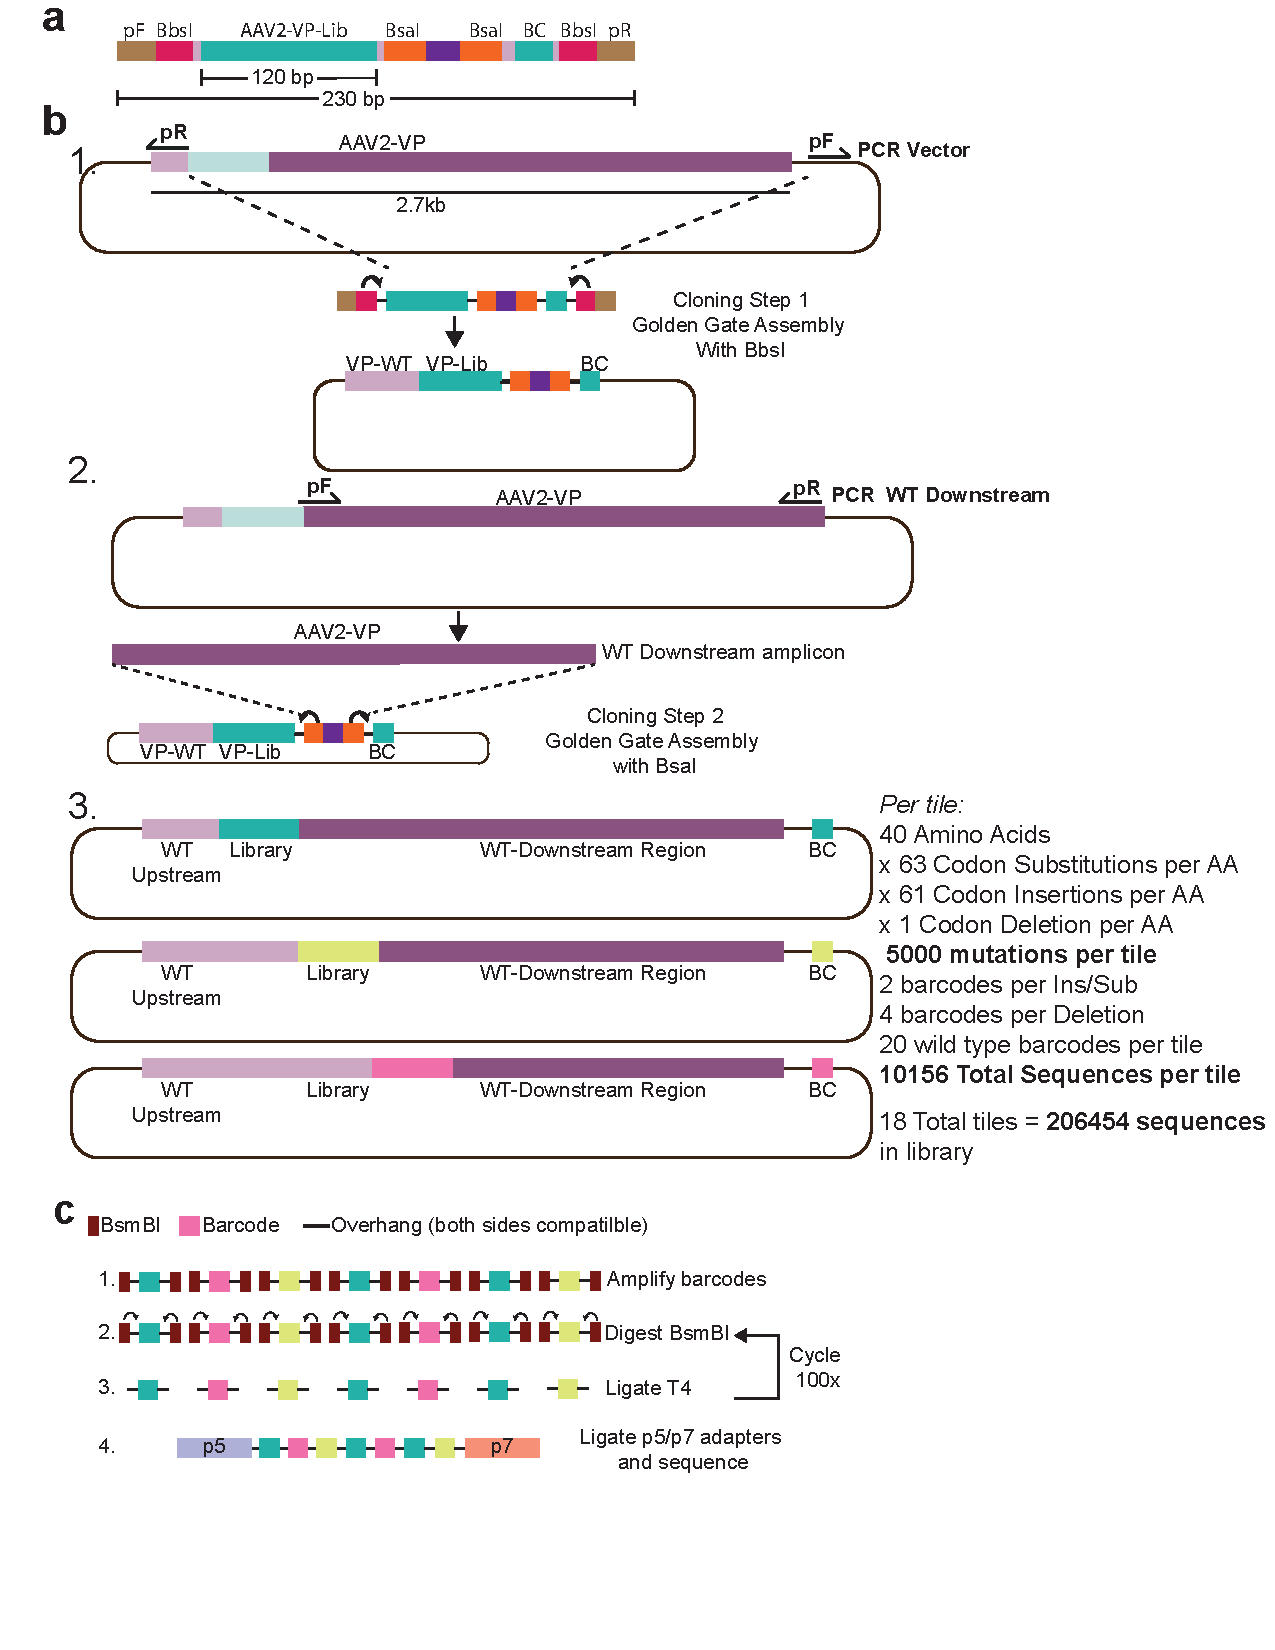
\includegraphics[width=\textwidth,height=\textheight]{figures/20180903_AAV2_supp_fig0_cloning.pdf}
\caption[Library cloning strategy and barcode ligation description]{Library cloning strategy and barcode ligation description. a, Diagram of a single chip oligo. b, Agilent array oligos are cloned into their respective locations using Type IIS restriction enzymes. In a successive step, the downstream gene region is added. c, Cloning introduced flanking BsmBI sites to barcodes, which cut into homologous 4 bp overhangs. Barcodes are cycled with Type IIS enzyme (BmsBI), ligase, and Illumina adapters, then libraries are amplified for sequencing via PCR.
\label{fig:Figure 6}}
\end{figure}

The full library was moved into 2 different ITR containing vector for packaging into viral particles: one using CMV as un upstream promoter (pCMV-AAV2-Lib) and one using AAV2-Rep as an upstream promoter (pRep-AAV2-Lib). Using Illumina sequencing we verified that 98.4\% of barcode variants were successfully assembled.

\subsection{Viral production assay}
Virus was produced was produced as previously described (25), with minor adjustments. Briefly, 293T cells were seeded into ten layer cell stacks (Corning 3270) for each experiment. Replicates of pCMV-AAV2-Lib and pPRep-AAv2-Lib were seeded in individual cell stacks. PEI transfection was performed with PEI:DNA mass ratio of 3:1 with 602.5 ug AAV-Rep (added only to pCMV-AAV2-Lib), 1017 ug pHelper, and 5ug AAV2 capsid library. Media (DMEM w/ Glutamax, Pen/Strep antibiotic, 5\% FBS) was changed after 24 hours, and 50\% media volume (500 mL) was added after 72 hours. After 5 days, cells were lysed with by adding NaCl to 150mM and incubating for 2 hours at 37C. The media cell mixture collected and allowed to sit overnight at 4C. The supernatant was separated and filtered through a 0.22uM filter (Corning 431098). 40\% PEG 8000 in dH20 was added to the virus material to a final concentration of 8\%, and incubated at 4C overnight. This material was spun at 4800g for 20 minutes, the pellet was collected and dissolved in 7mL PBS. The material was then subjected to iodixanol gradient purification29, concentrated using a spin concentrator (Millipore UFC910024), and frozen at -80C. 

\subsection{Barcode ligation}
Barcodes from plasmid (1 ng/uL) or virus samples (1uL of 1e10 vg/uL virus prep) were amplified using PCR from flanking primer sequences. The amplified product was purified, mixed with Illumina adapters with homologous overhangs at 50:1 barcode:adapter molar ratios, put into a GGA reaction (BsmBI and T4 ligase, NEB), allowed to cycle 100x overnight (Fig. S1) (16C 5 min, 37C 5 min). This material was then amplified to add Illumina annealing adapters and indexes and sequenced using the NextSeq platform. 

\subsection{Packaging Assay Analysis}
Library plasmids and virus samples were sequenced using barcode ligation as described above. Individual mutant counts (cm) were determined using custom scripts. Packaging counts across replicates are summed before computing frequencies. The frequency of a mutant in the virus pool (fv) or the plasmid pool (fv)  was calculated as f = cm / ∑cm. Selection of each mutant in the virus pool was calculated as s = fv / fp. This selection value was then normalized to the wild-type replicate selection value  as s’ = s / swt, where swt  is the median WT selection value calculated normalization. Selection values for WT replicates, stop codons in VP3 and stop codons in VP/VP2 were separated into their respective sets and their distributions compared using a Mann-Whitney U test. The mean selection value for residue insertions at each position was calculated and plotted onto the 1lp3 pdb structure17 using custom PyMOL scripts. For serotype comparisons, AAV1-12, AAV.hu43 and AAV.hu48, were aligned to AAV2 RefSeq using Geneious (standard alignment parameters). The alignment was used to determine which residues were contained in other serotypes at the relevant positional comparison. Residues within variable regions were defined as previously described18,19, and p-values were calculated using both a Mann-Whitney U test and a Kolmogorov–Smirnov test.

\begin{figure}
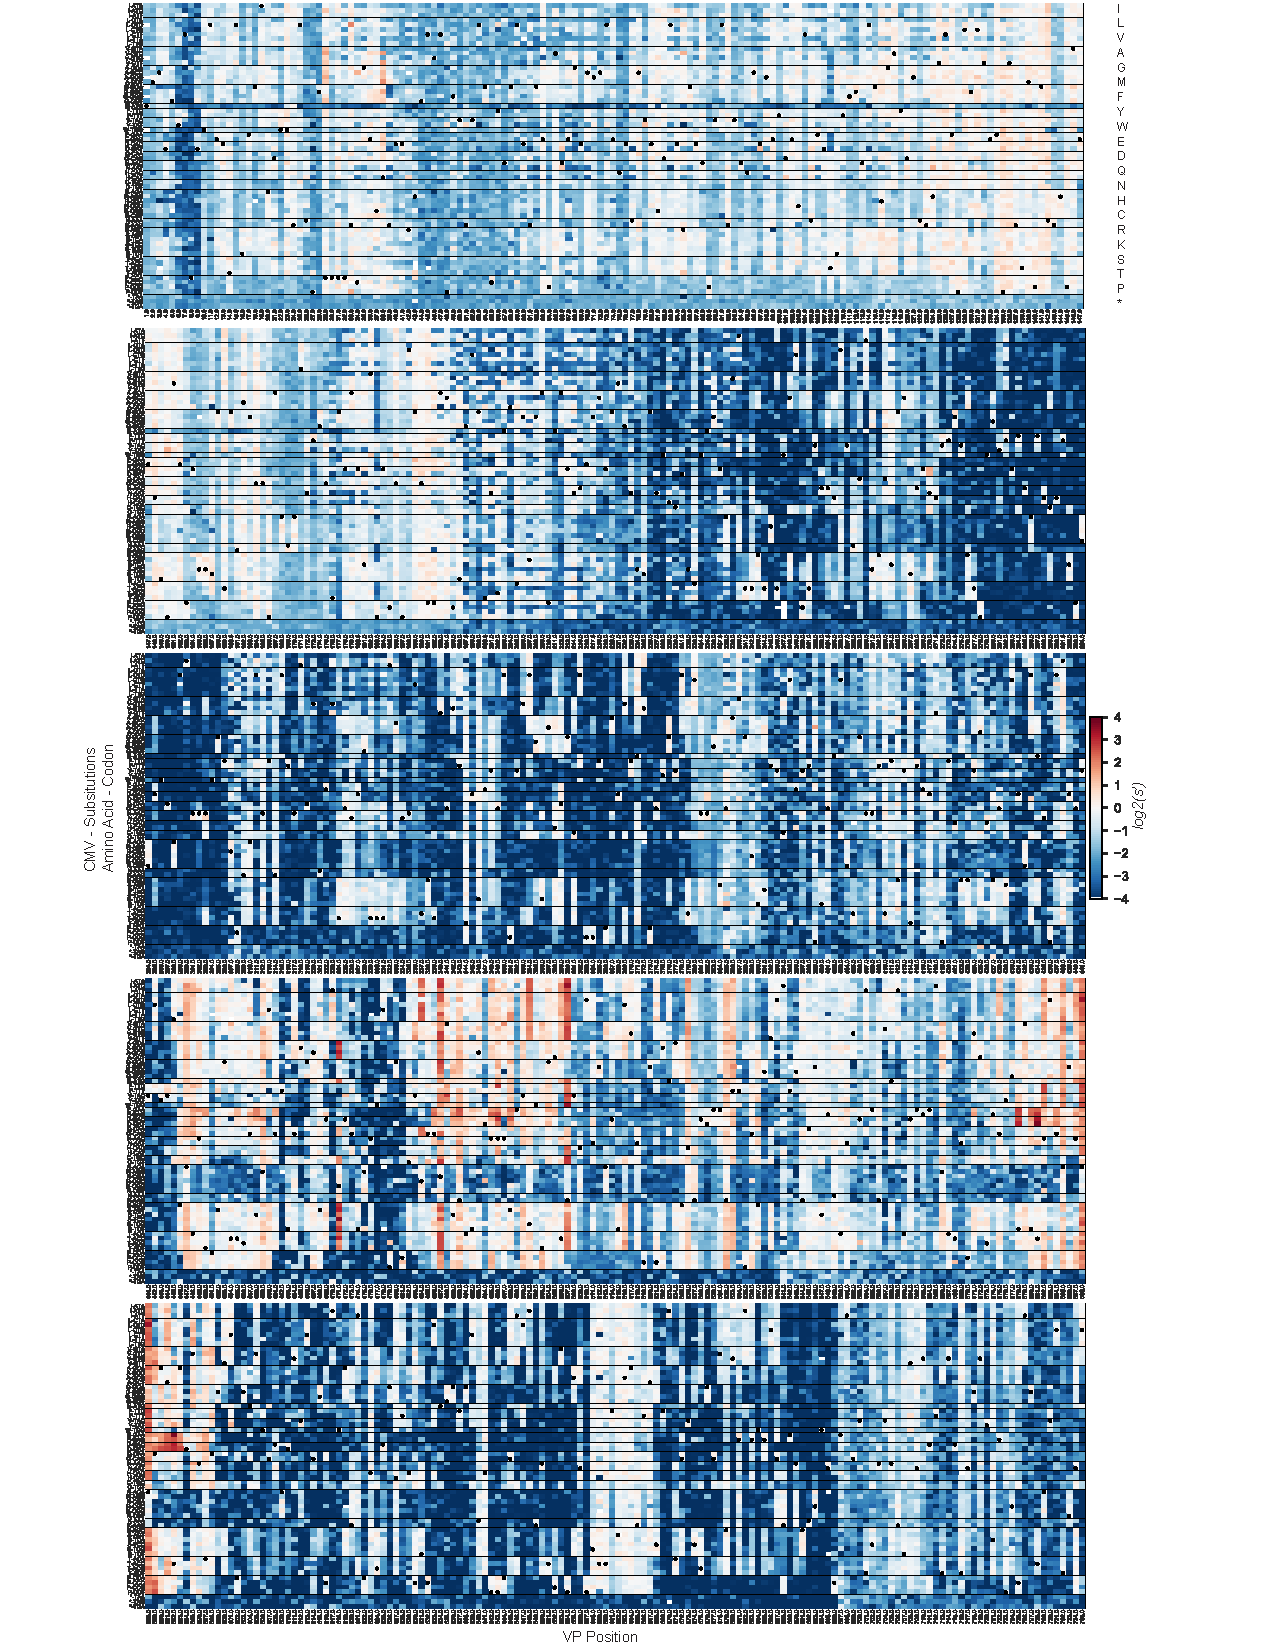
\includegraphics[width=\textwidth,height=\textheight]{figures/20180903_AAV2_supp_fig1_CMV_subs.pdf}
\caption[All codon substitutions for the CMV AAV2-Cap  library]{All codon substitutions for the CMV AAV2-Cap  library
\label{fig:Figure 6}}
\end{figure}

\begin{figure}
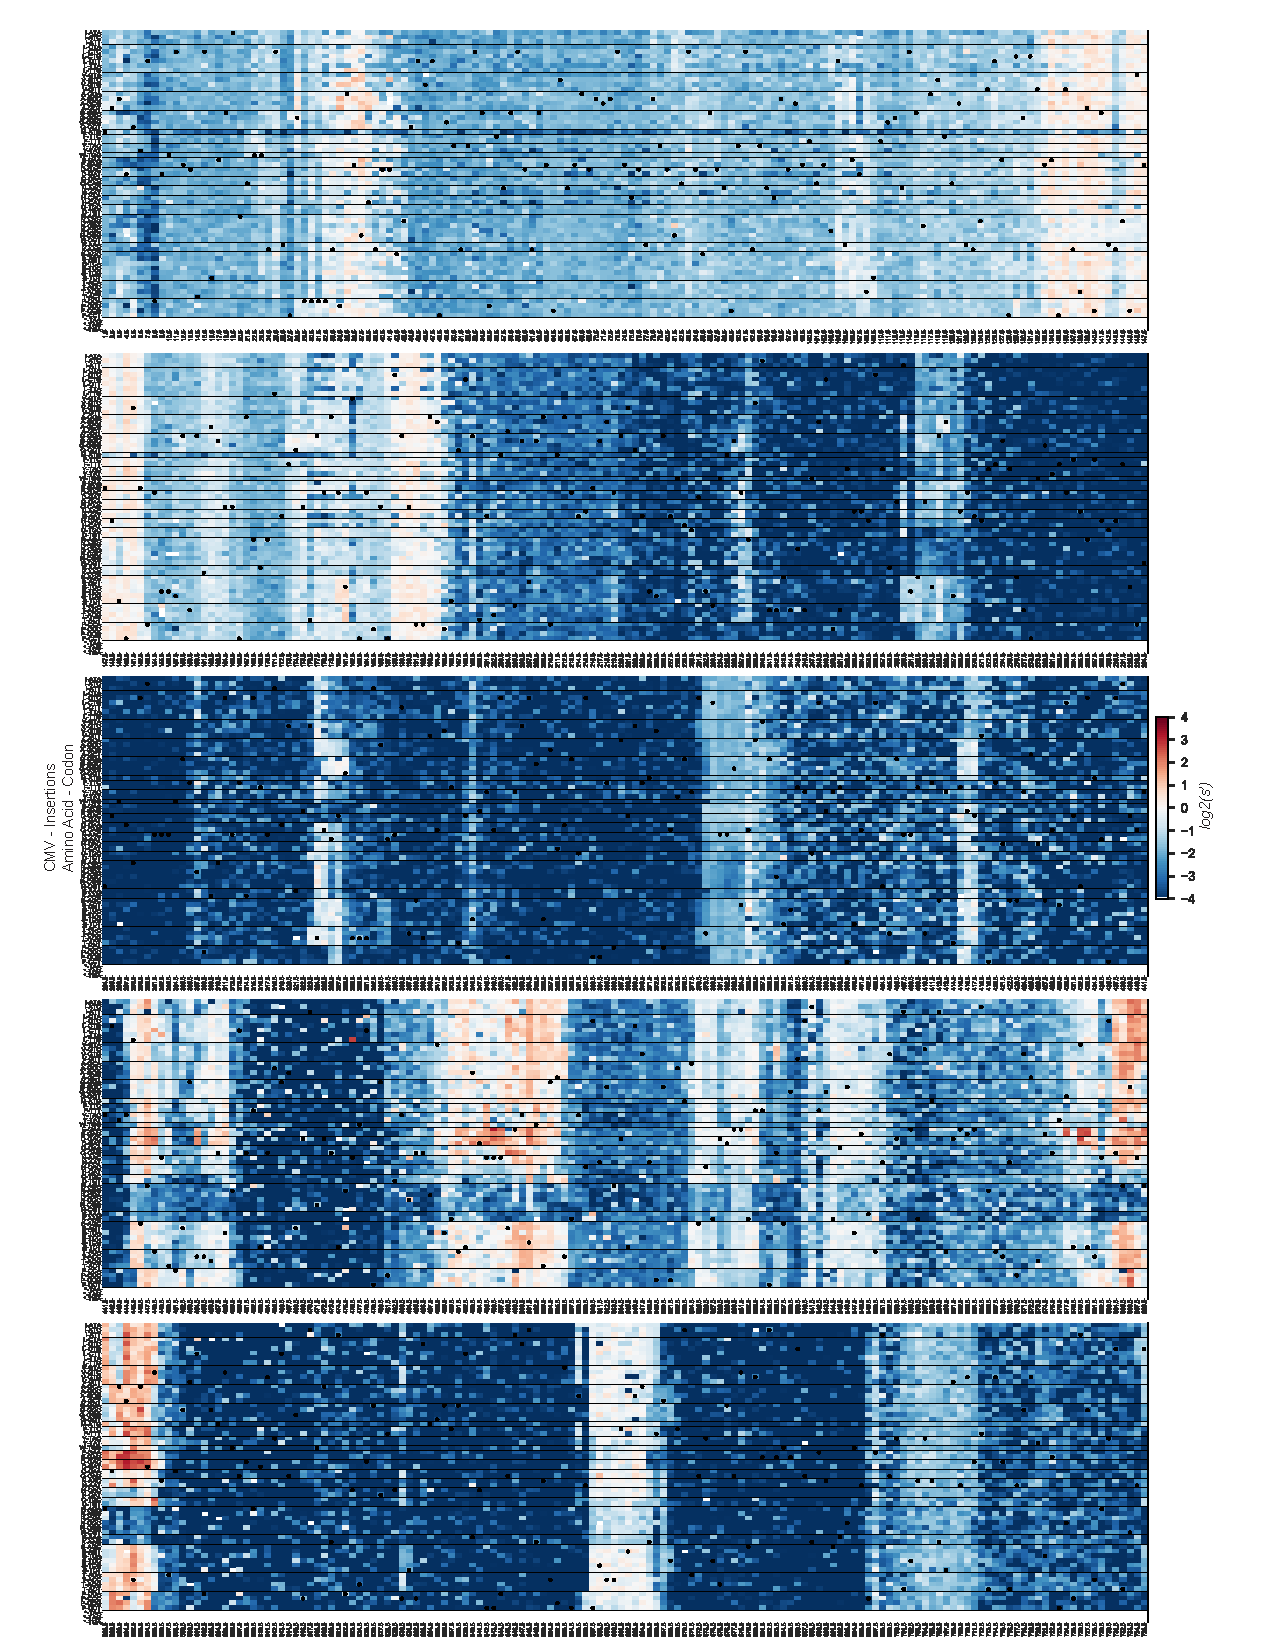
\includegraphics[width=\textwidth,height=\textheight]{figures/20180903_AAV2_supp_fig2_CMV_ins.pdf} 
\caption[All codon insertions for the CMV AAV2-Cap  library]{All codon insertions for the CMV AAV2-Cap  library
\label{fig:Figure 7}}
\end{figure}

\begin{figure}
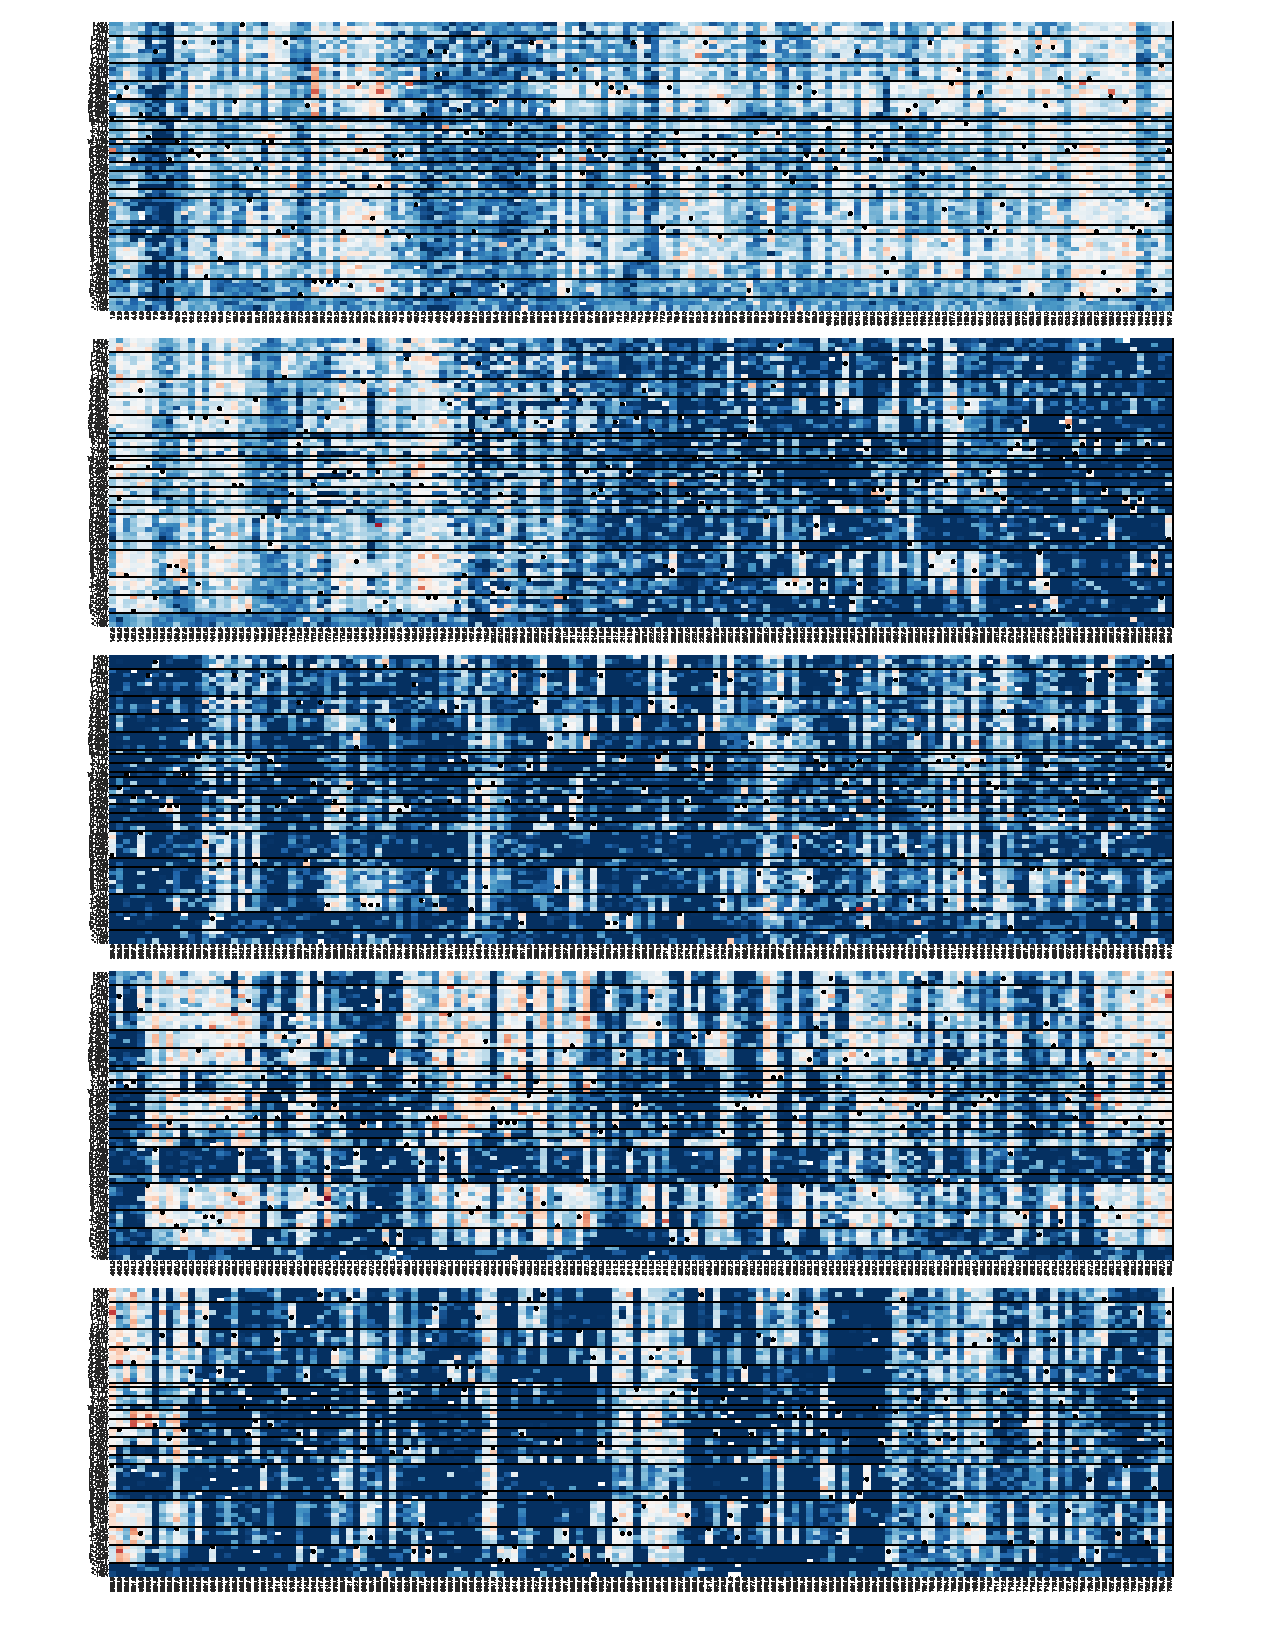
\includegraphics[width=\textwidth,height=\textheight]{figures/20180903_AAV2_supp_fig3_Rep_subs.pdf} 
\caption[All codon substitutions for the Rep AAV2-Cap  library]{All codon substitutions for the Rep AAV2-Cap  library
\label{fig:Figure 8}}
\end{figure}

\begin{figure}
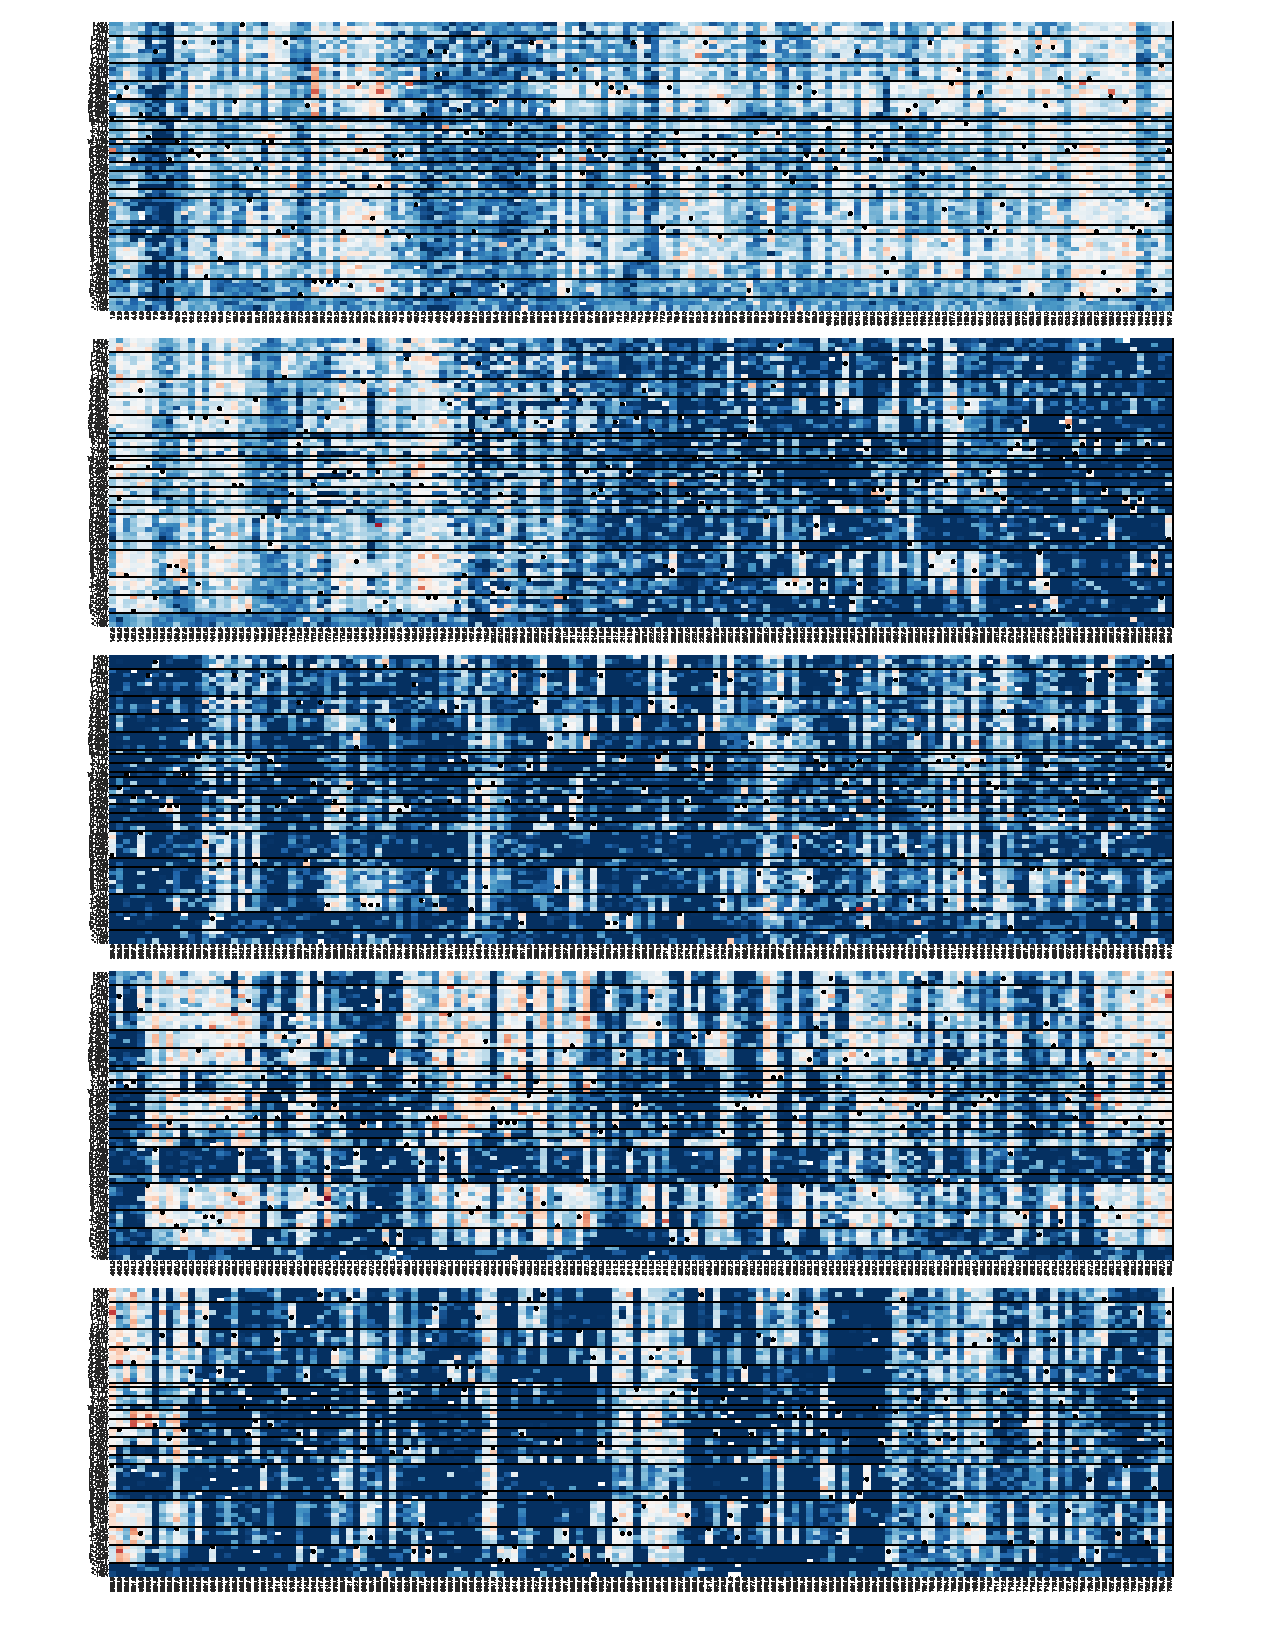
\includegraphics[width=\textwidth,height=\textheight]{figures/20180903_AAV2_supp_fig3_Rep_subs.pdf} 
\caption[All codon insertions for the Rep AAV2-Cap  library]{All codon insertions for the Rep AAV2-Cap  library
\label{fig:Figure 9}}
\end{figure}


\subsection{Thermostability assay}
Individual AAV2 library samples (~1e10 vg) were incubated at varying temperatures (intervals: 55, 60, 65, 66, 67, 68, 69, 70, 80, 90 degrees Celsius) in 10uL PBS for 30 minutes. To this material, 1uL DNaseI was added and incubated for 1 hour, then heat killed at 65C for 15 minutes. The samples were then PCR amplified, subjected to barcode ligation and sequenced.  

For analysis frequency of each mutant (ftm) was calculated and selection calculated in comparison to virus as above. The ratio of mutants contained below a threshold of log(s’) < -2.5 were calculated at each temperature. The Tm  of AAV2 (~65) was chosen for structure plotting.
The ratio was plotted as a heatmap on the structure using PyMOL and the PyMOL color mapping “gray\_yellow\_orange\_red”.  

\subsection{A20 antibody neutralization assay}
AAV2 Rep-Cap library was incubated with A20 antibody (Fitzgerald, 10R-A110a). 50ug of lyophilized A20 antibody was resuspended in 1mL H2O to make a concentrated stock solution. hAd5 adenovirus stock solution (ATCC-VY 1516) was made by filtering from media from HEK293T cells infected and lysed with hAD5 according to ATCC instructions. Antibody was prepared in a 2-fold dilution series in 1mL DMEM, ranging from 1x to 32x, where 1x was 625ng antibody in 2mL DMEM media. These concentrations were chosen so the 50\% inhibition of AAV2 was achieved approximately in the middle of the dilution series, based upon luciferases assays with WT AAV2. A20 dilution in 0.5mL DMEM was added to 1e10vg virus library in 500uL DMEM and incubated for 30 minutes at room temperature, then added on to 1e6 HEK293T cells growing in wells of 6-well plates, and 1mL of fresh DMEM with 10\% FBS was added. Cells were incubated 36 hours at 37C, then media was aspirated, cells were washed with PBS, then 1/10,000x dilution of hAd5 stock was added. Cell lysis was visible after 5 days. Cells were collected, pelleted, and viral DNA was purified using a Qiagen mini-prep alkaline lysis kit. The resulting DNA was PCR amplified, barcodes were ligated and sequenced on a NextSeq 5000. 

For analysis, the 2x dilution of A20 antibody was used. Frequency of virus in the antibody pool (fab) was calculated as above, and selection was calculated as s = fab/fv, and normalized to wild-type as described above. Positions known to bind to A20 from cryo-EM structures20 were separated (A20 Interacting), and this distribution was compared to the distribution of all other positions (Other Residues) using a Kolmogorov–Smirnov test. The fraction of residues with log2(s’) > 2.5 were calculated using custom python scripts.  

\subsection{Mouse Biodistribution assay}
1e12 vg of AAV2 library was injected retro orbitally into 8 mice. Blood was drawn after 1 hour from each mouse injected and frozen on dry ice. After two weeks, tissue samples were extracted and frozen on dry ice. Approximately 150 mg of each organ was ground using disposable mortar and pestle (Kimble Chase 749625-0010). DNA was purified using alkaline lysis (26). DNA was PCR amplified and sequenced using barcode ligation.

\begin{figure}
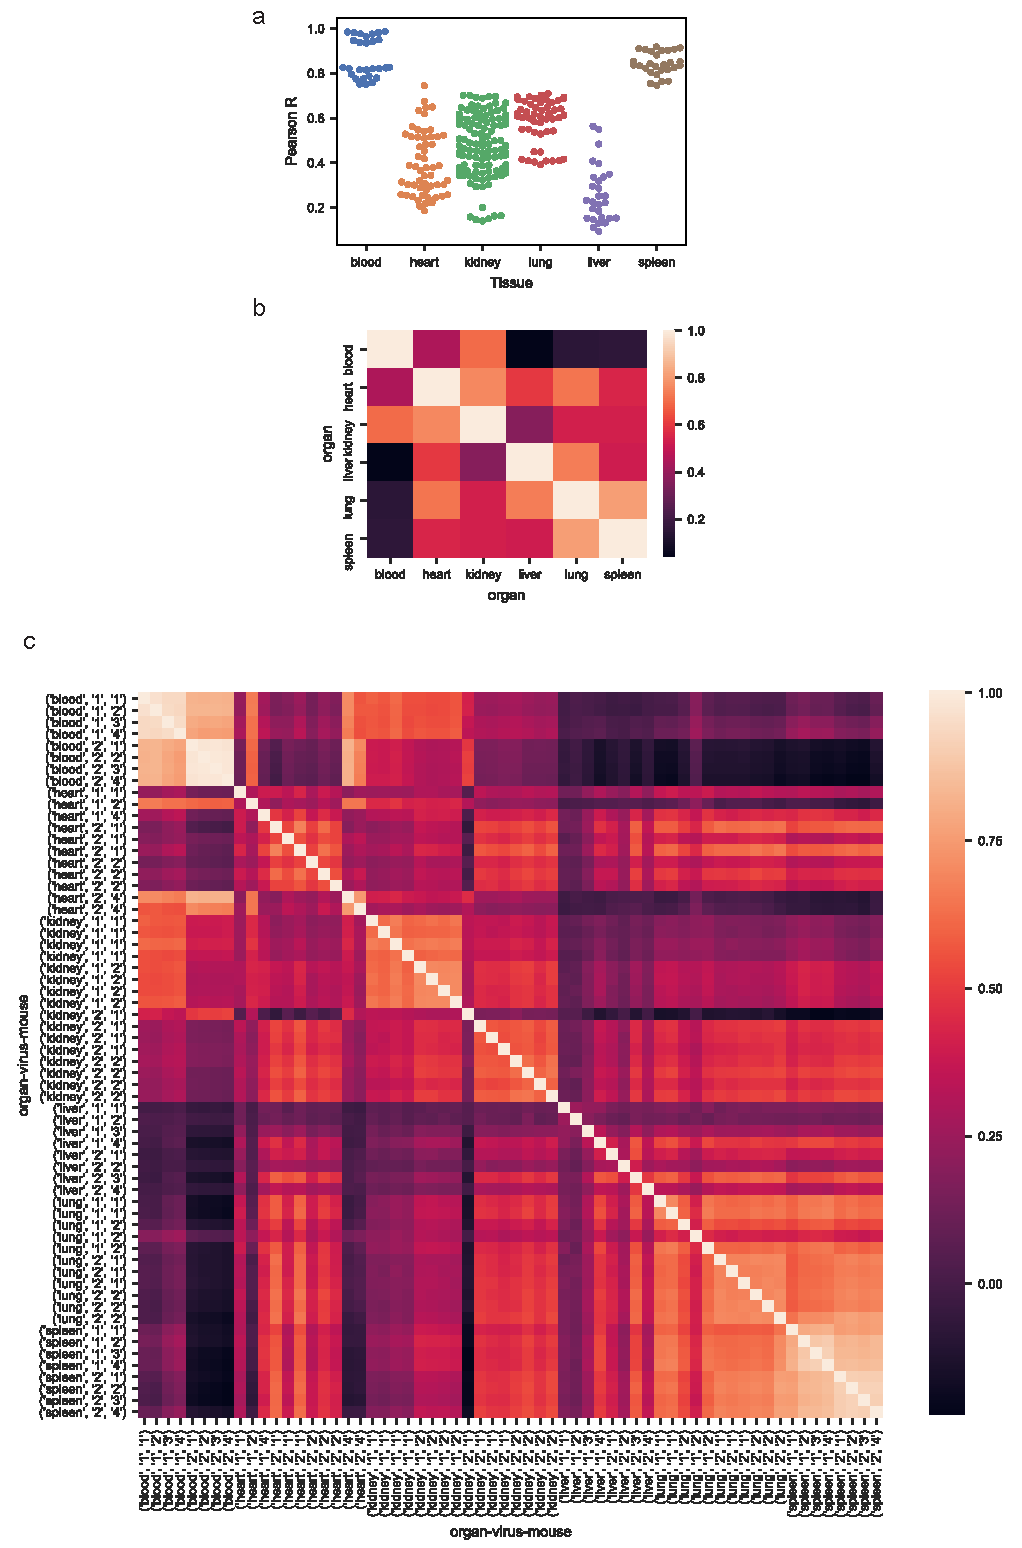
\includegraphics[width=\textwidth,height=\textheight,keepaspectratio]{figures/20190610AAV2_sup_figx_mouse_tissue_data_correalation.pdf} 
\caption[Pearson correlations of all mouse tissue selection values across replicates]{Pearson correlations of all mouse tissue selection values across replicates a) intra tissue b) inter tissue c) all replicates
\label{fig:Figure 10}}
\end{figure}

For analysis, the frequency of each mutant (ft) in a tissue, and normalized selection values were calculated as above. Replicate tissue prep selection values were compared (Fig. S9) to ensure strong correlation. For PCA, the dataset was first filtered to contain only mutants with s’package > 0.5. Mutants were further filtered to contain only mutants which had -1 < log2(s’t ) or log2(s’t) > 1 for at least one tissue, to remove mutants which had no effect across any tissues. The resulting mutants median selection value for each tissue were put into a PCA analysis using python packaging sklearn. Mutant Classes were selected using a combination of PC values and median tissue selection values, as well as kmeans cluster association (Fig S10). Residues contained in each Class were plotted on the structure using PyMOL and custom scripts. 



\subsection{Mouse Validation Assay}
Mutants (N705W, ins261S,R471K,T567Q,R588T) selected for mouse validation were individually cloned and virus variants were produced packaging eGFP and tittered (concentrations calculated against qPCR standards). WT AAV2 was independently produced with mKate and titered. Each mutant was pooled approximately equally with WT virus and injected in 3 mouse replicates (approx 5e11 total vg per mouse). 1 week later tissues were processed and viral DNA extracted with alkaline lysis. The input pool was titered using IDT qPCR probes against mKate (WT-AAV2) and eGFP (mutant-AAV) as was the AAV DNA from the tissue sample. First, we computed the ratio of mutant-AAV to WT-AAV2 from the qPCR values for both samples. Selection was determined by computing the ratio of these two values (tissue/input) which determines if the mutant if enriched or depleted in a given tissue in direct comparison to the wild type: S’ = tissue(Cqmutant\_AAV/Cqwt\_AAV2) / virus(Cqmutant\_AAV/Cqwt\_AAV2).

\subsection{MAAP Validation}
Calculation of the Frameshift Score (FS): For MAAP validation, a table of mutations made in the MAAP/AAP +1 frame (single base shift forward from VP) was created. When mutating a single codon in the VP frame, two MAAP frame mutations are possible. Any amino acid mutation with at least one codons that created a stop codon in MAAP/AAP frame was taken for use in this analysis. For these amino acids, the difference between MAAP stop codons vs non-stop MAAP codons was calculated across all codons synonymous for that amino acid. FS was the average of these differences across all amino acids. To determine significance of a given FS, a null model was created by permuting the selection values of all synonymous codons for amino-acids containing one or more MAAP stop (105 random permutations), and the average selection difference between MAAP stops and non-stops was computed. The difference values were then smoothed using a rolling window of 10 positions.  The distribution of smoothed values was used to calculate a z-score, and the z-score value for the un-shuffled data was used to create an estimated p-value using the gaussian cumulative distribution function.

For MAAP validation, three constructs were created. These constructs all had MAAP in the native background upstream gene context (with Rep functionally intact), however the VP1 start codon were mutated to ensure no VP gene expression interference. For the ∆Start, VP-P27-CCT codon was mutated to CCC. For the ∆Stop, VP-P32-CCT codon was mutated to ATA (V), making an early stop codon in MAAP. Virus production was performed as described above, however pREP was substituted for the pREP-MAAP constructs in their respective cases. p-values for the pREP-MAAP wild type construct were also calculated as described above. 

For western blot, a 3xFLAG tag was added downstream to pREP-MAAP, pREP-MAAP∆Start and pREP∆Stop. These constructs were transfected into 10cm dish of 293T cells using PEI in a 3:1 ratio with pREP-MAAP plasmid DNA (4.4 ug), either with or without pHelper (8.8 ug). Cells were collected into RIPA buffer with protease inhibitors, quantified with BCA assay (Pierce 23225), denatured using LDS and B-mercaptoethanol, and  ~120ug was run on Tris-glycine 4-20\% gel (Life XP04202BOX). Proteins were transferred to nitrocellulose membrane using I-blot system, and stained using Mouse M2 anti-FLAG 1:1000 (Sigma F3165), and mouse m2 anti GAPDH (Sigma ). Gels were then stained with secondary anti-mouse HRP, and visualized at multiple exposure (1, 2, and 5 seconds). 

For imaging, cells were plated on chamber slides (ThermoScientific 154917) and transfected with pHelper, pRep-MAAP-FLAG (Fig SX) or pRep-MAAP-GFP (Fig 3), and an mCherry-ITR plasmid (control) and with pCap (Fig 3), thus containg all requirements for AAV production. Negative controls were plated with only pHelper and mCherry-ITR. Cells were fixed in 4\% PFA for 30 mins, and then stained with Mouse M2 anti-FLAG primary antibody (Sigma F3165), Alex452–antiMouse secondary antibody, Hoechst stain, and visualized on using confocal microscopy. In the case of cells transfected with pRep-MAAP-GFP, cells were fixed as above and imaged directly using 63x confocal objective. Image deconvolution was performed in Huygens software. 

% \texttt{This is a line of code.}

% % % Requires fltpage2 package
% \begin{FPfigure}
% \includegraphics[width=\textwidth]{figures/fullpage.pdf}
% \caption[Short figure name.]{This is a full page figure using the FPfigure command. It takes up the whole page and the caption appears on the preceding page. Its useful for large figures. Harvard's rules about full page figures are tricky, but you don't have to worry about it because we took care of it for you. For example, the full figure is supposed to have a title in the same style as the caption but without the actual caption. The caption is supposed to appear alone on the preceding page with no other text. You do't have to worry about any of that. We have modified the fltpage package to make it work. This is a lengthy caption and it clearly would not fit on the same page as the figure. Note that you should only use the FPfigure command in instances where the figure really is too large. If the figure is small enough to fit by the caption than it does not produce the desired effect. Good luck with your thesis. I have to keep writing this to make the caption really long. LaTex is a lot of fun. You will enjoy working with it. Good luck on your post doctoral life! I am looking forward to mine. \label{fig:myFullPageFigure}}
% \end{FPfigure}
% \afterpage{\clearpage}

